The power supply layer is one of the most important layers because it provides stable power supply
to the cart. The parts in this subsystem are responsible for powering every other subsystem and any
external tools or equipment.

\subsection{DEEP CYCLE BATTERY}
A rechargeable battery that will provide consistent power up to 12 V.
\begin{figure}[h!]
	\centering
 	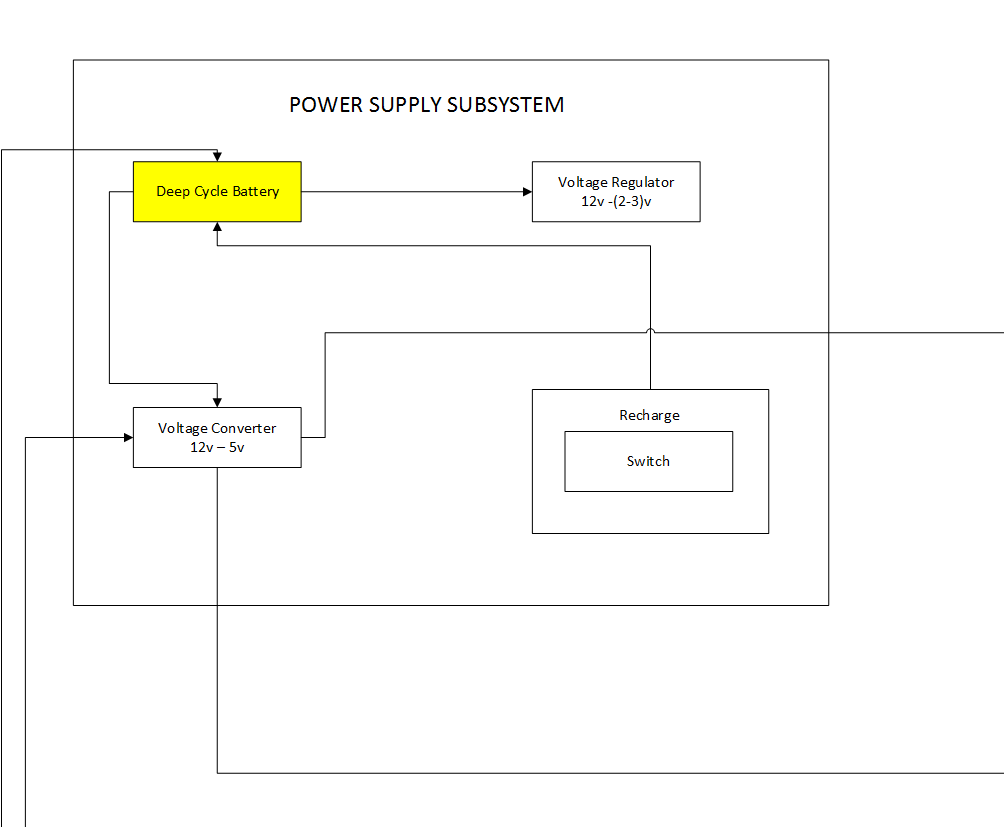
\includegraphics[width=0.60\textwidth]{images/battery}
 \caption{Deep Cycle Battery Subsystem description diagram}
\end{figure}

\subsubsection{ASSUMPTIONS}
\begin{itemize}
\item The battery is charged.
\item The battery is properly connected to the cart
\item The battery is fully functional
\item The battery is connected to the cart at all times
\end{itemize}

\subsubsection{RESPONSIBILITIES}
The deep cycle battery subsystem responsibilities are as follows:
\begin{itemize}
\item Provide stable power supply to the other subsystems after being converted from 12v to 5v by the voltage converter.
\item Enable stable power to external tools and equipment after being converted from 12V to 2 - 3V through the voltage regulator.
\end{itemize}

\subsubsection{SUBSYSTEM INTERFACES}
\begin {table}[H]
\caption {Deep cycle battery subsystem interfaces} 
\begin{center}
    \begin{tabular}{ | p{1cm} | p{6cm} | p{3cm} | p{3cm} |}
    \hline
    ID & Description & Inputs & Outputs \\ \hline
    \ N/A & Power integrated power supply & \pbox{3cm}{N/A} & \pbox{3cm}{Voltage regulator }  \\ \hline
    \ N/A & Power electronic components & \pbox{3cm}{N/A} & \pbox{3cm}{Voltage converter}  \\ \hline
    \ N/A & Safety killswitch & \pbox{3cm}{Killswitch} & \pbox{3cm}{N/A}  \\ \hline
    \ N/A & Safety manual mode & \pbox{3cm}{Manual-mode switch} & \pbox{3cm}{N/A}  \\ \hline
    \end{tabular}
\end{center}
\end{table}

\subsection{VOLTAGE REGULATOR}
The voltage regulator is designed to convert the 12V voltage from the deep cycle battery to 2 - 3V and it will mainly be used to power up external tools and equipment.
\begin{figure}[h!]
	\centering
 	\includegraphics[width=0.60\textwidth]{images/voltageRegulator}
 \caption{Voltage Regulator Subsystem description diagram}
\end{figure}

\subsubsection{ASSUMPTIONS}
Assumptions made are as follows:
\begin{itemize}
\item The voltage from the battery will be 12v.
\item The voltage required fro external tools and equipment will be between 2-3v.
\end{itemize}

\subsubsection{RESPONSIBILITIES}
\begin{itemize}
\item To enable and regulate constant voltage level for powering external tools and supplies.
\end{itemize}

\subsubsection{SUBSYSTEM INTERFACES}
\begin {table}[H]
\caption {Voltage Regulator Subsystem Interfaces} 
\begin{center}
    \begin{tabular}{ | p{1cm} | p{6cm} | p{3cm} | p{3cm} |}
    \hline
    ID & Description & Inputs & Outputs \\ \hline
    \ N/A & Receive power & \pbox{3cm}{Deep Cycle Battery} & \pbox{3cm}{N/A }  \\ \hline
    \end{tabular}
\end{center}
\end{table}


\subsection{RECHARGE}
The Recharge subsystem will be used to to ensure that Smart Cart will be charged without having too much electricity going to the battery or other cart components
\begin{figure}[h!]
	\centering
 	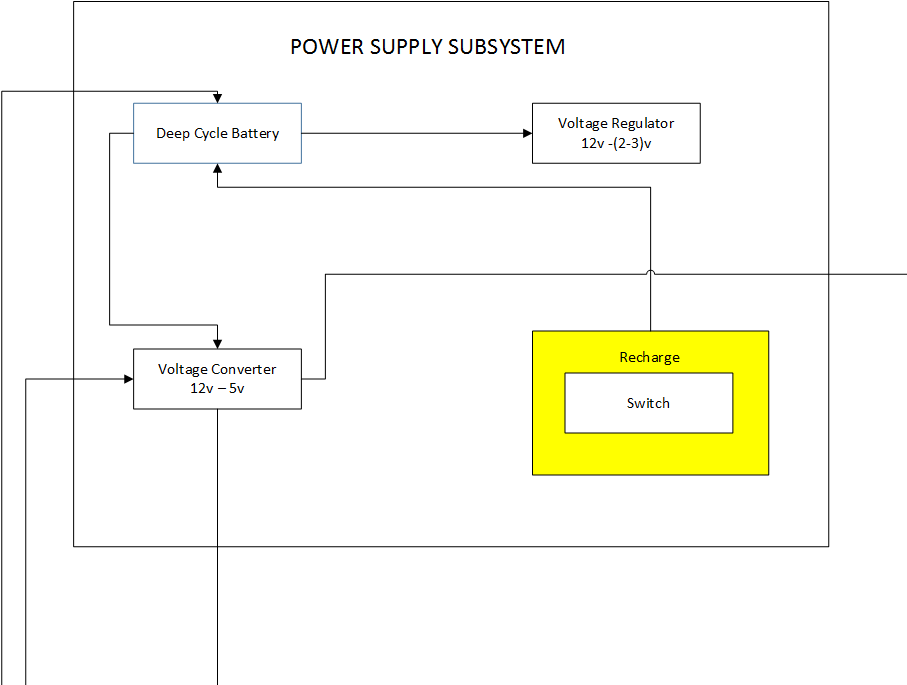
\includegraphics[width=0.60\textwidth]{images/recharge}
 \caption{Recharge Subsystem}
\end{figure}

\subsubsection{ASSUMPTIONS}
Assumptions are as follows:

\begin{itemize}
\item The Recharge subsystem will ensure the safety of the tools and equipment.
\end{itemize}

\subsubsection{RESPONSIBILITIES}
The responsibilities of the Recharge subsystem are as follows:

\begin{itemize}
\item A switch will disable the battery from the powering the Smart Cart components while it is being charged
\end{itemize}

\subsubsection{SUBSYSTEM INTERFACES}
\begin {table}[H]
\caption {Recharge Subsystem Interfaces} 
\begin{center}
    \begin{tabular}{ | p{1cm} | p{6cm} | p{3cm} | p{3cm} |}
    \hline
    ID & Description & Inputs & Outputs \\ \hline
    \ N/A & Switch o safety & \pbox{3cm}{Switch} & \pbox{3cm}{Deep cycle battery}  \\ \hline
    \end{tabular}
\end{center}
\end{table}

\subsection{VOLTAGE CONVERTER}
The voltage regulatlor is designed to convert the 12V from the deep cycle battery to a 2-3V to be used to power up smart cart equipment
\begin{figure}[h!]
	\centering
 	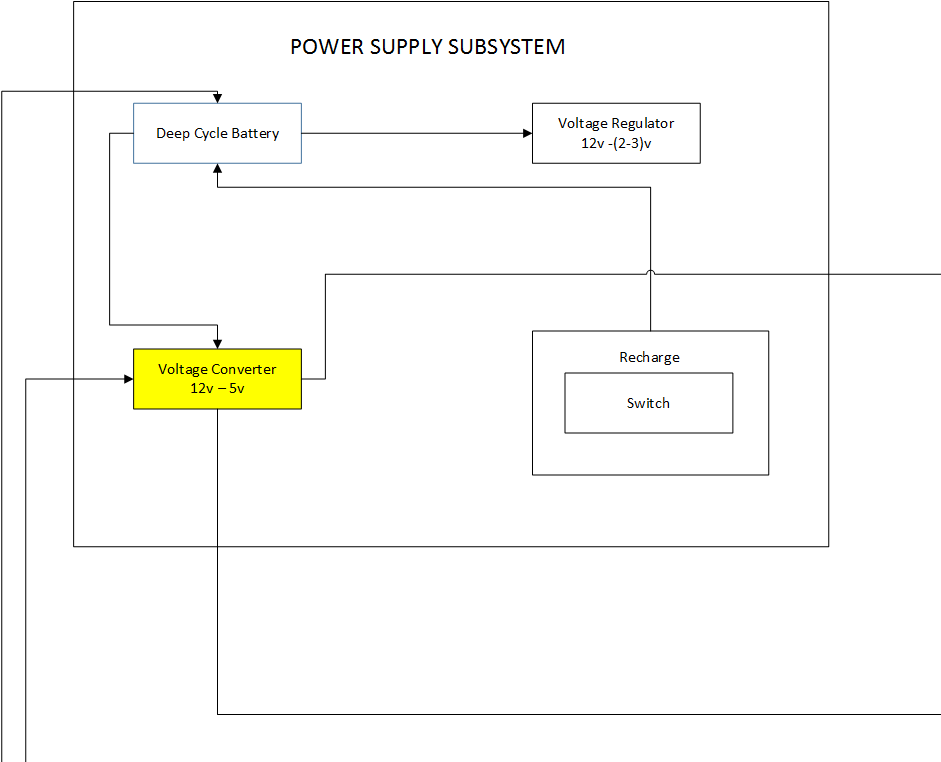
\includegraphics[width=0.60\textwidth]{images/voltageconverter}
 \caption{Voltage Converter Subsystem}
\end{figure}

\subsubsection{ASSUMPTIONS}
Assumptions made are as follows:
\begin{itemize}
\item The voltage from the battery will be 12V.
\item The voltage required by the cart's components will be 5V
\end{itemize}

\subsubsection{RESPONSIBILITIES}
The voltage converter subsystem responsibilities are as follows:
\begin{itemize}
\item Enable stable power to the other subsystems, which include the crab drive system and image processing after being converted from 12V to 5V through the voltage converter.
\end{itemize}

\subsubsection{SUBSYSTEM INTERFACES}

\begin {table}[H]
\caption {Voltage Converter Subsystem Interfaces} 
\begin{center}
    \begin{tabular}{ | p{1cm} | p{6cm} | p{3cm} | p{3cm} |}
    \hline
    ID & Description & Inputs & Outputs \\ \hline
    \ N/A & Receive Power &\pbox{3cm}{Deep Cycle battery} & \pbox{3cm}{N/A} \\ \hline
    \ N/A & Safety Manual Mode & \pbox{3cm}{Manual-mode switch} & \pbox{3cm}{Crab-drive system Imaging and Navigation }  \\ \hline
    \end{tabular}
\end{center}
\end{table}
